\documentclass[11pt,a4paper]{article}

\usepackage[margin=2.5cm]{geometry}
\usepackage{amsmath,amssymb}
\usepackage{graphicx}
\usepackage{booktabs}
\usepackage{hyperref}
\usepackage{natbib}
\usepackage{setspace}
\usepackage{caption}
\usepackage{enumitem}
\usepackage{microtype}
\usepackage{subcaption}
\usepackage{float}

\hypersetup{colorlinks=true, linkcolor=blue, citecolor=blue, urlcolor=blue}
\setstretch{1.15}
\bibliographystyle{apalike}

\title{%
  From Labour-Supply Shock to Economic Adjustment:\\
  A Stylised Agent-Based Model of Immigration, Wages, and Firm Dynamics}

\author{Scott Brodie Forsyth\\[0.5em]\small Independent Researcher}
\date{July 2026}

\begin{document}
\maketitle

% Auto-generated by experiment.py — do not edit by hand
\newcommand{\NReplicates}{50}
\newcommand{\MZeroShortWage}{-0.05}
\newcommand{\MSixShortWage}{2.32}
\newcommand{\MZeroLongWage}{-0.34}
\newcommand{\MSixLongWage}{6.41}
\newcommand{\LowSkillShortWage}{0.682}
\newcommand{\HighSkillShortWage}{0.898}
\newcommand{\DemandContrib}{1.33}
\newcommand{\EntryContrib}{1.11}
\newcommand{\InnovContrib}{0.09}
\newcommand{\MZeroEmpShort}{45.2}
\newcommand{\MSixEmpShort}{92.7}
\newcommand{\MZeroUnempShort}{56.9}
\newcommand{\MSixUnempShort}{7.9}
\newcommand{\MZeroShortWageSE}{0.07}


\begin{abstract}
\noindent
Empirical studies disagree on whether immigration lowers native wages because they embed different adjustment margins: some hold job counts fixed, others allow product demand, firm creation, capital, occupational specialisation, and innovation to respond.
This paper develops a structurally transparent agent-based labour-market model and nests seven specifications---from a pure labour-supply benchmark (\emph{M0}) to a full general-equilibrium model with innovation (\emph{M6})---to identify \emph{when}, \emph{through which mechanisms}, and \emph{for whom} immigration-induced supply shocks matter.
Calibration uses stylised aggregate moments---employment gaps, wage differentials, and migrant self-employment rates---drawn from broad patterns reported in the OECD and immigration-literature \citep{borjas2016,dustmann2013,oecd2024entrepreneurship,peri2016}.
A balanced 5\% labour-force shock is simulated with \NReplicates{} stochastic replicates per mechanism level.
Under \emph{M0}, the short-run native wage index changes by \MZeroShortWage{} percentage points on average (95\% interval includes zero); native employment falls to \MZeroEmpShort{}\% and economy-wide unemployment rises to \MZeroUnempShort{}\%.
Under \emph{M6}, the wage index \emph{rises} by \MSixShortWage{} percentage points in the short run and \MSixLongWage{} percentage points in the long run (8--12 years), while short-run native employment is \MSixEmpShort{}\% and unemployment \MSixUnempShort{}\%; native employment nonetheless declines gradually over the post-shock horizon.
Mechanism decomposition attributes \DemandContrib{} percentage points of short-run wage change to activating local consumption demand (\emph{M0}$\rightarrow$\emph{M1}), \EntryContrib{} to firm entry (\emph{M1}$\rightarrow$\emph{M2}), and \InnovContrib{} to innovation (\emph{M5}$\rightarrow$\emph{M6}).
The exercise does \emph{not} estimate a causal effect for any observed economy; it shows that fixed-job and dynamic general-equilibrium thought experiments can be nested within one framework, and that the \emph{sign} of wage and employment outcomes depends critically on which margins are active and on the time horizon.
\end{abstract}

\noindent\textbf{Keywords:} immigration; agent-based model; search and matching; firm dynamics; mechanism decomposition; general equilibrium

\noindent\textbf{JEL codes:} J15; J23; J31; J61; C63; F22

\section{Introduction}
\label{sec:intro}

Immigration expands the workforce.
In the simplest textbook model, an exogenous increase in labour supply along a downward-sloping short-run demand curve reduces wages for competing workers \citep{borjas2003,borjas2016}.
Yet much of the empirical literature finds smaller, null, or even positive effects on average native wages once markets are defined broadly and adjustment is allowed time to unfold \citep{card1990,ottaviano2012,peri2016}.
The disagreement is not primarily about arithmetic; it is about \emph{structure}: which margins---product demand, vacancy creation, capital accumulation, occupational reallocation, entrepreneurship, spatial mobility, innovation---are held fixed in the thought experiment.

Recent theoretical work formalises this distinction in search environments where immigrants may accept lower wages, be hired preferentially, and thereby induce firms to open additional vacancies \citep{albert2021}.
Spatial evidence shows that immigrants respond to local labour demand far more elastically than natives, attenuating geographic wage dispersion \citep{cadenakovak2016,monras2020}.
Expenditure channels matter because migrants consume locally while remitting part of their income \citep{cheremukhin2024}.
Firm-level analyses show that immigration can shift entry and production organisation, particularly for high-skilled inflows \citep{waugh2018}.
Over longer horizons, immigration may raise innovation and productivity sufficiently to dominate short-run supply effects \citep{terry2026}.

This paper asks:
\begin{quote}
  \emph{Under which structural conditions does an immigration-induced labour-supply shock affect native wages and employment in the short run, and when do endogenous adjustments in demand, firm entry, capital, occupational specialisation, and innovation offset or reverse those effects?}
\end{quote}

The contribution is methodological and diagnostic.
An agent-based model (ABM) is built in which workers (natives and migrants), firms, and implicit households interact through multi-task production, search-and-matching frictions, and optional general-equilibrium feedbacks \citep{epstein2006,railsback2019}.
Seven nested specifications (\emph{M0}--\emph{M6}) activate mechanisms sequentially.
Counterfactual immigration shocks vary in size, skill composition, substitutability, and macroeconomic state.
Outcomes are reported by skill group and time horizon (0--2, 3--7, and 8--12 years).

Parameters are chosen to reproduce stylised moments consistent with high-income OECD labour markets \citep{borjas2016,dustmann2013,peri2016}, not to replicate any single country's administrative data.
The model is a \emph{computational laboratory}: an artificial economy in which mechanisms can be switched on or off to diagnose comparative statics.

Section~\ref{sec:background} summarises evidence.
Section~\ref{sec:model} presents the model.
Section~\ref{sec:design} describes the experimental design.
Section~\ref{sec:results} reports results.
Section~\ref{sec:limits} states limitations.
Section~\ref{sec:conclusion} concludes.

\section{Conceptual background and hypotheses}
\label{sec:background}

\subsection{Why estimates diverge}

\citet{borjas2016} catalogues how differences in skill definition, geographic market, native complementarity, and capital adjustment drive opposing conclusions.
Partial-equilibrium studies that treat job counts as fixed tend to find more negative competition effects \citep{borjas2003}.
General-equilibrium models with product-demand feedback, heterogeneous tasks, or endogenous technology often find smaller average wage losses and sometimes gains for complementary natives \citep{peri2016,peri2009,ottaviano2012}.

Task-based frameworks emphasise that immigrants and natives may not compete within the same occupational cell even when they share a broad education category \citep{peri2009}.
Immigrants frequently experience occupational downgrading---working below the skill level suggested by formal qualifications---which shifts competition toward specific tasks rather than entire skill tiers \citep{dustmann2013,borjas2016}.

\subsection{Adjustment margins}

\textbf{Job creation.}
In search models, immigration lowers effective hiring costs when migrants accept lower reservation wages.
Firms respond by posting more vacancies, creating a job-creation offset to job competition \citep{albert2021}.

\textbf{Demand.}
Immigrants earn wages and consume locally; remittances leak expenditure abroad \citep{cheremukhin2024}.

\textbf{Firm dynamics.}
Immigration changes factor costs and market size, shifting entry and exit \citep{waugh2018}.

\textbf{Innovation.}
Immigration can raise local innovation through diversity and scale \citep{terry2026}.

\textbf{Spatial equilibrium.}
Immigrants relocate toward high-demand areas, diffusing local shocks \citep{cadenakovak2016,monras2020}.

\subsection{Hypotheses}

\begin{enumerate}[label=\textbf{H\arabic*}. , nosep]
  \item \textbf{Short-run competition:} Immigration raises labour-market congestion when capital and firm numbers are fixed (\emph{M0}); wage-index changes are small and statistically indistinguishable from zero in this parameterisation.
  \item \textbf{Demand adjustment:} Local consumption attenuates or reverses negative wage effects (\emph{M1} vs.\ \emph{M0}).
  \item \textbf{Firm dynamics:} Firm entry and capital accumulation reduce labour-market congestion (\emph{M2}, \emph{M3}).
  \item \textbf{Complementarity:} Natives in higher skill tiers have higher wage-index levels; inflow skill mix shifts aggregate outcomes only modestly under \emph{M6} (\emph{M4}).
  \item \textbf{Entrepreneurship:} Migrant entrepreneurship accelerates job creation (\emph{M5}).
  \item \textbf{Dynamic reversal:} Average wage-index effects may shift from negligible under \emph{M0} to positive in the long run when demand, firm entry, and innovation operate (\emph{M6}).
\end{enumerate}

\section{Model}
\label{sec:model}

\subsection{Overview}

Figure~\ref{fig:schematic} in Appendix~\ref{app:schematic} depicts the architecture.
Time is discrete, $t = 0,1,\ldots,T$.
There are $R$ regions, $S$ skill sectors, and $Q$ task types.
Worker $i$ is characterised by origin $g_i \in \{\text{native},\text{migrant}\}$, skill $s_i$, occupation $o_i$, productivity $a_i$, reservation wage $r_i$, employment status $e_i \in \{0,1\}$, and location $z_i$.
Migrants additionally carry remittance rates, skill transferability, entrepreneurship propensity, and occupational downgrading risk.

Firms operate in a region--sector cell, hold capital $K_j$, post vacancies, and employ natives $N_{jq}$ and migrants $M_{jq}$ in each task $q$.

\subsection{Production}

Firm $j$ produces with nested CES technology:
\begin{equation}
  \label{eq:production}
  Y_j = A_j K_j^{\alpha}
  \left[
    \sum_{q=1}^{Q} \omega_q L_{jq}^{\frac{\sigma-1}{\sigma}}
  \right]^{\frac{\sigma}{\sigma-1}},
\end{equation}
where $A_j$ is productivity, $\alpha \in (0,1)$ the capital share, $\omega_q$ task weights, and $\sigma>0$ the elasticity of substitution across tasks.

Within each task, native and migrant labour combine as
\begin{equation}
  \label{eq:task}
  L_{jq} =
  \left[
    \theta_q N_{jq}^{\frac{\rho_q-1}{\rho_q}}
    + (1-\theta_q) M_{jq}^{\frac{\rho_q-1}{\rho_q}}
  \right]^{\frac{\rho_q}{\rho_q-1}}.
\end{equation}
When $\rho_q \to \infty$, natives and migrants are perfect substitutes within the task; lower $\rho_q$ implies stronger complementarity \citep{peri2009,peri2016}.

\subsection{Labour market}

Each period: (i)~household demand; (ii)~vacancy posting; (iii)~separations; (iv)~unemployed-to-vacancy matching; (v)~production and pricing; (vi)~firm entry/exit; (vii)~capital adjustment; (viii)~occupational mobility, innovation, and periodic relocation.

Matching follows a stylised search protocol \citep{pissarides2000}: unemployed workers apply to vacancies in their region and occupation; matches form with probability increasing in the wage offer relative to reservation productivity.
Immigrants' lower reservation wages imply higher job-finding rates, consistent with \citet{albert2021}.

\subsection{Product demand (\emph{M1})}

When \emph{M1} is active, consumption feeds back to sectoral demand.
Disposable income for household $h$ satisfies
\begin{equation}
  \label{eq:consumption}
  C_{ht} = c\,\max\!\bigl(Y_{ht} - R_{ht} - T_{ht},\, 0\bigr) + C_0,
\end{equation}
where $Y_{ht}$ is labour income, $R_{ht}$ remittances (zero for natives), $T_{ht}$ taxes, and $c$ the marginal propensity to consume.
Sectoral demand indices scale firm sales expectations, prices, and vacancy targets.

\subsection{Firm dynamics (\emph{M2}--\emph{M3})}

Potential entrants observe expected profits $\mathbb{E}[\pi_{st}]$, entry cost $F_s$, and demand $D_{st}$:
\begin{equation}
  \label{eq:entry}
  P(\text{entry}_{st}) =
  \Lambda\!\left(
    \gamma_0 + \gamma_1 \mathbb{E}[\pi_{st}] - \gamma_2 F_s + \gamma_3 D_{st}
  \right),
\end{equation}
where $\Lambda(x)=1/(1+e^{-x})$ is the logistic function.
Incumbent firms exit after persistent losses; capital accumulates when utilisation and profits are high (\emph{M3}).

\subsection{Specialisation, entrepreneurship, and innovation}

\emph{M4}: employed natives upgrade toward their skill tier \citep{peri2009}.
\emph{M5}: unemployed migrants create firms at OECD-calibrated rates \citep{oecd2024entrepreneurship}.
\emph{M6}: innovation success raises $A_j$ with probability increasing in local skill diversity and R\&D labour \citep{terry2026}.

\subsection{Immigration shock}

After a 10-year burn-in, migrants arrive exogenously at $t=10$, raising the workforce by $\Delta L/L \in \{1\%, 3\%, 5\%, 10\%\}$ with varying skill mixes.
Subsequent location choices are endogenous.

\section{Experimental design and calibration}
\label{sec:design}

\subsection{Mechanism ladder}

\begin{align*}
  \text{M0}: & \ \text{labour supply only (fixed firms, capital, demand)} \\
  \text{M1}: & \ \text{M0} + \text{local consumption demand} \\
  \text{M2}: & \ \text{M1} + \text{firm entry and exit} \\
  \text{M3}: & \ \text{M2} + \text{capital adjustment} \\
  \text{M4}: & \ \text{M3} + \text{task specialisation} \\
  \text{M5}: & \ \text{M4} + \text{migrant entrepreneurship} \\
  \text{M6}: & \ \text{M5} + \text{innovation}.
\end{align*}
The incremental contribution of mechanism $k$ is $\Delta \bar{w}^{\text{M}_k} - \Delta \bar{w}^{\text{M}_{k-1}}$, where $\Delta \bar{w}$ is the mean change in a native skill-wage index relative to the pre-shock baseline.

\subsection{Calibration targets}

Table~\ref{tab:calibration} lists stylised calibration targets informed by published immigration and labour-market research.
Parameters not directly identified are set by simulated-method-of-moments logic to approximate burn-in moments.
In the current implementation, pre-shock employment rates under \emph{M6} exceed the native-employment target in Table~\ref{tab:calibration}; the artificial economy is therefore stylised rather than tightly identified.
Hold-out validation against observed historical shocks is reserved for future work (Section~\ref{sec:limits}).

\begin{table}[htbp]
  \centering
  \small
  \caption{Stylised calibration targets (literature-informed)}
  \label{tab:calibration}
  \begin{tabular}{@{}p{0.38\textwidth}p{0.14\textwidth}p{0.36\textwidth}@{}}
    \toprule
    Moment & Target & Source \\
    \midrule
    Native employment rate & 81.5\% & stylised OECD range \citep{borjas2016} \\
    Migrant employment rate & 67.0\% & immigrant employment gap \citep{dustmann2013} \\
    Migrant labour-force share & 12\% & stylised \citep{peri2016} \\
    Native--migrant wage ratio & 1.12 & wage-gap literature \citep{dustmann2013,borjas2016} \\
    Migrant self-employment (relative) & elevated & \citet{oecd2024entrepreneurship} \\
    Remittance share of migrant income & 5\% & literature benchmark \\
    \bottomrule
  \end{tabular}
\end{table}

\subsection{Implementation and replication}

The model is implemented in Python with vectorised worker and firm arrays.
Defaults: $N=2{,}500$ workers, $R=5$ regions, $S=3$ skill sectors, 10-year burn-in, 12-year post-shock horizon.
Each main cell uses \NReplicates{} stochastic replicates; the research design envisions 500 replicates with global sensitivity analysis \citep{saltelli2008} as a scalability target.
Documentation follows the ODD protocol \citep{grimm2010}.
Code, calibration files, result CSVs, and replication scripts are available at \url{https://github.com/sbf-developer/migration-labour-computational-simulation}.

\section{Results}
\label{sec:results}

\subsection{Summary}

Three findings organise the simulation output.
First, under \emph{M0} (fixed jobs and demand), a 5\% immigration shock produces negligible average wage-index change but severe labour-market congestion (Table~\ref{tab:employment}).
Second, activating demand and firm entry (\emph{M1}--\emph{M2}) accounts for most of the shift to positive wage-index changes; later mechanisms (\emph{M3}--\emph{M6}) contribute little at the aggregate level in this parameterisation.
Third, under \emph{M6}, rising wage indices coexist with a gradual decline in native employment share over the post-shock horizon (Figure~\ref{fig:paths}), so wages and employment are not interchangeable summary statistics.

\subsection{Mechanism ladder}

Table~\ref{tab:results} and Figure~\ref{fig:ladder} report native wage-index changes after a balanced 5\% immigration shock.
Under \emph{M0}---labour supply only, with fixed firm count, capital, and product demand---the short-run wage index changes by \MZeroShortWage{} percentage points on average (standard error $\approx$\MZeroShortWageSE{} pp; 95\% interval includes zero).
The main \emph{M0} effect is not a large wage cut but severe matching congestion: native employment falls to \MZeroEmpShort{}\% and economy-wide unemployment rises to \MZeroUnempShort{}\% in the short run (Table~\ref{tab:employment}, Figure~\ref{fig:ladder}b).
Activating local consumption demand (\emph{M1}) shifts the short-run wage effect by \DemandContrib{} percentage points and restores employment to roughly pre-shock levels, supporting \textbf{H2} in direction though the magnitude should be interpreted cautiously (Section~\ref{sec:limits}).
Firm entry (\emph{M1}$\rightarrow$\emph{M2}) contributes a further \EntryContrib{} percentage points in the short run.
By \emph{M6}, the short-run wage effect is \emph{positive} (\MSixShortWage{} pp) and the long-run effect (years 8--12) reaches \MSixLongWage{} pp; short-run native employment is \MSixEmpShort{}\% but declines over the post-shock horizon (Figure~\ref{fig:paths}), so wages and employment need not move in the same direction.

% Auto-generated results table
\begin{table}[htbp]
  \centering
  \caption{Native wage-index change (\%) by mechanism level: balanced 5\% shock}
  \label{tab:results}
  \begin{tabular}{lcc}
    \toprule
    Model & Short run (0--2 yr) & Long run (8--12 yr) \\
    \midrule
    M0 & -0.05 (0.07) & -0.34 (0.11) \\
    M1 & 1.28 (0.04) & 4.63 (0.06) \\
    M2 & 2.39 (0.06) & 6.66 (0.12) \\
    M3 & 2.30 (0.06) & 6.38 (0.10) \\
    M4 & 2.30 (0.06) & 6.38 (0.10) \\
    M5 & 2.23 (0.05) & 6.23 (0.10) \\
    M6 & 2.32 (0.06) & 6.41 (0.10) \\
    \bottomrule
  \end{tabular}
  \begin{minipage}{0.92\textwidth}
    \small\emph{Note:} Entries are mean native skill-wage-index changes (\%) relative to the pre-shock baseline, with 95\% replicate standard errors in parentheses. $N=\NReplicates{}$ replicates per cell.
  \end{minipage}
\end{table}


% Auto-generated employment table
\begin{table}[htbp]
  \centering
  \caption{Native employment and unemployment after a balanced 5\% shock}
  \label{tab:employment}
  \small
  \begin{tabular}{@{}lcccc@{}}
    \toprule
    Model & Native emp.\ (short) & Unemp.\ (short) & Native emp.\ (long) & Comment \\
    \midrule
    M0 & 45.2\% (0.3) & 56.9\% (0.3) & 27.2\% (0.3) & Severe congestion; fixed jobs \\
    M1 & 97.4\% (0.1) & 2.9\% (0.1) & 97.8\% (0.0) & Demand restores matching \\
    M6 & 92.7\% (0.2) & 7.9\% (0.3) & 86.4\% (0.4) & Wages up; employment drifts down over time \\
    \bottomrule
  \end{tabular}
  \begin{minipage}{0.92\textwidth}
    \small\emph{Note:} Short run = years 0--2 after shock; long run = years 8--12. Unemployment is economy-wide. 95\% replicate standard errors in parentheses.
  \end{minipage}
\end{table}


\begin{figure}[H]
  \centering
  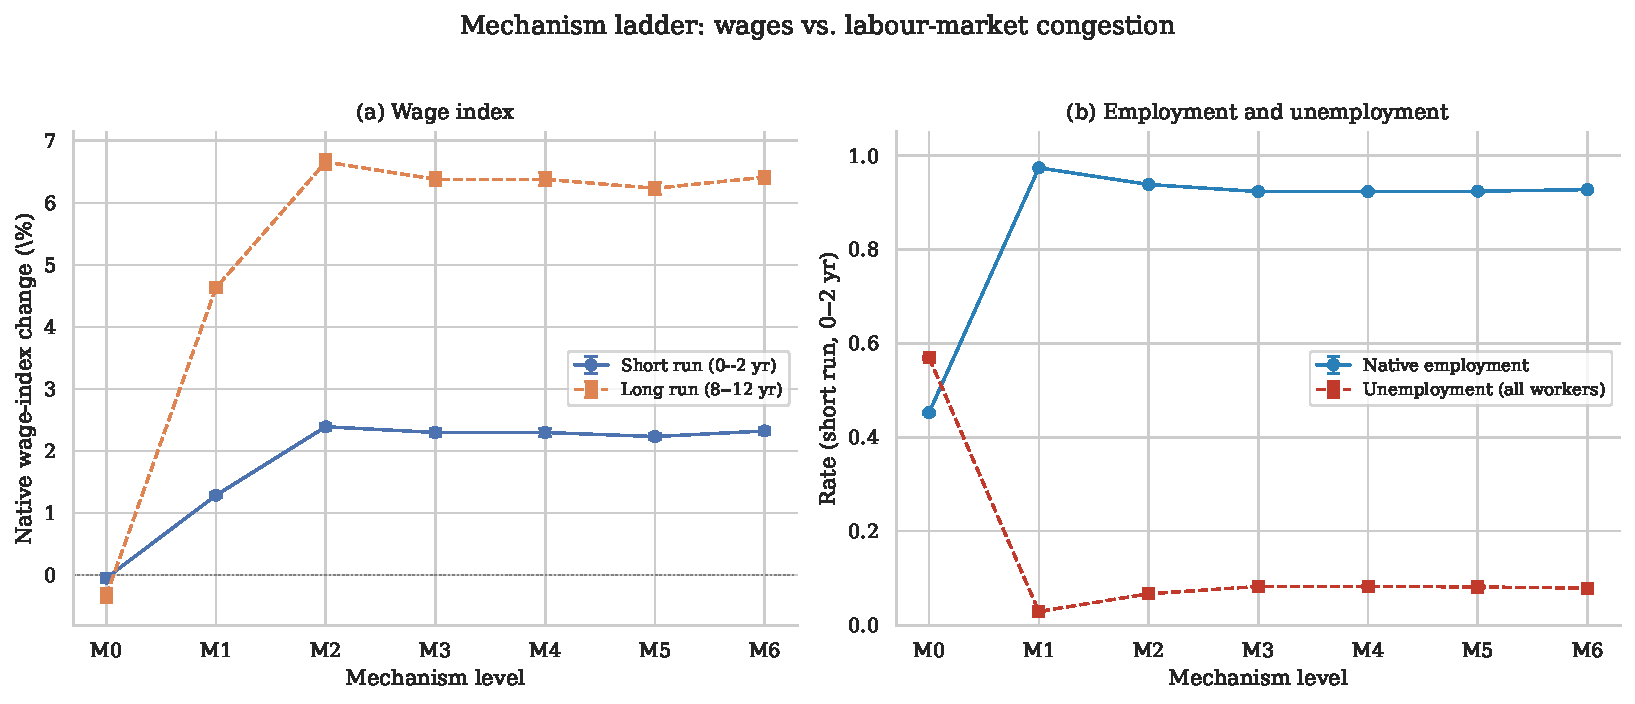
\includegraphics[width=\textwidth]{../figures/fig2_mechanism_ladder.pdf}
  \caption{Mechanism ladder after a balanced 5\% immigration shock at $t=10$. Panel (a): native wage-index change (\%). Panel (b): short-run native employment and economy-wide unemployment. Error bars: 95\% confidence intervals across \NReplicates{} replicates.}
  \label{fig:ladder}
\end{figure}

\begin{figure}[H]
  \centering
  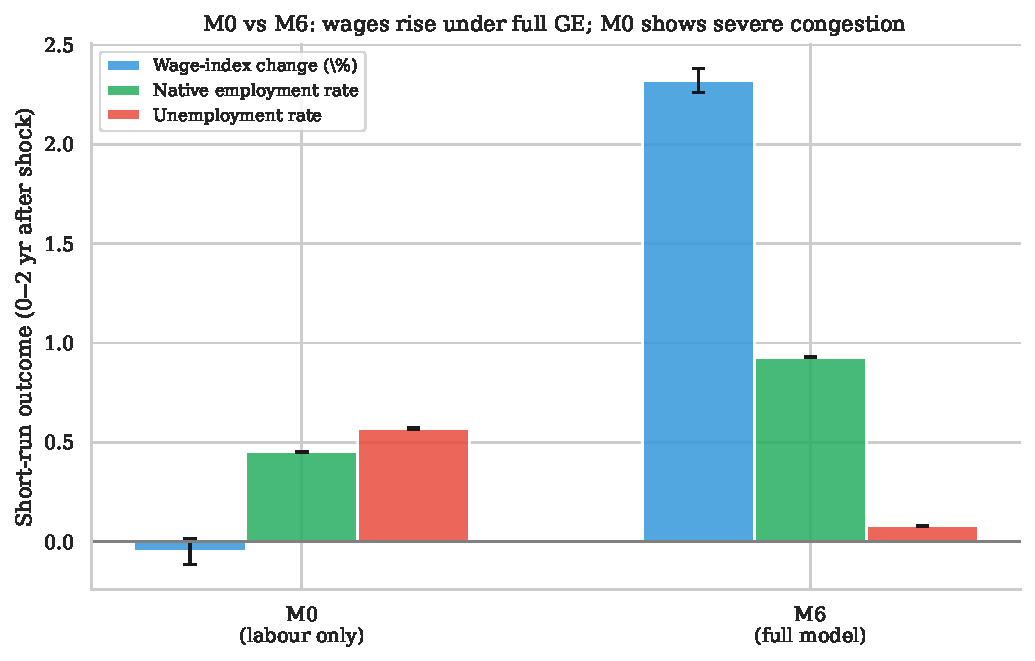
\includegraphics[width=0.88\textwidth]{../figures/fig7_m0_m6_comparison.pdf}
  \caption{M0 vs.\ M6: short-run wage-index change, native employment, and unemployment after a 5\% shock. Under fixed margins (\emph{M0}), congestion dominates; under full adjustment (\emph{M6}), wages rise while employment remains high in the short run but drifts down over time (Figure~\ref{fig:paths}).}
  \label{fig:m0m6}
\end{figure}

Figure~\ref{fig:decomp} decomposes incremental mechanism contributions.
The largest single step is typically \emph{M0}$\rightarrow$\emph{M1} (demand), followed by \emph{M1}$\rightarrow$\emph{M2} (firm entry).

\begin{figure}[H]
  \centering
  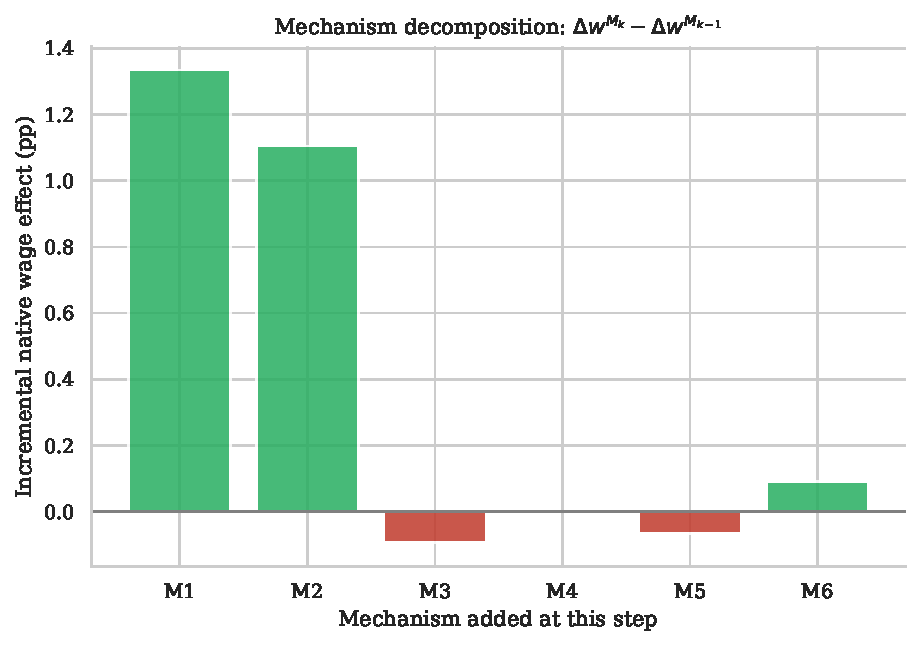
\includegraphics[width=0.88\textwidth]{../figures/fig3_decomposition.pdf}
  \caption{Mechanism decomposition: $\Delta \bar{w}^{\text{M}_k} - \Delta \bar{w}^{\text{M}_{k-1}}$ (percentage points, short run).}
  \label{fig:decomp}
\end{figure}

\subsection{Dynamic paths}

Figure~\ref{fig:paths} plots aggregate trajectories under \emph{M6}.
After the shock, the native wage index rises monotonically as general-equilibrium margins adjust; output per capita also increases.
Native employment falls from roughly 96\% pre-shock to about 86\% by year 20, and unemployment rises from about 4\% to 14\% over the same horizon---a pattern not visible in wage-index panels alone.
This is qualitatively consistent with long-run positive wage effects in \citet{terry2026}, though the model is not calibrated to any specific historical episode.

\begin{figure}[H]
  \centering
  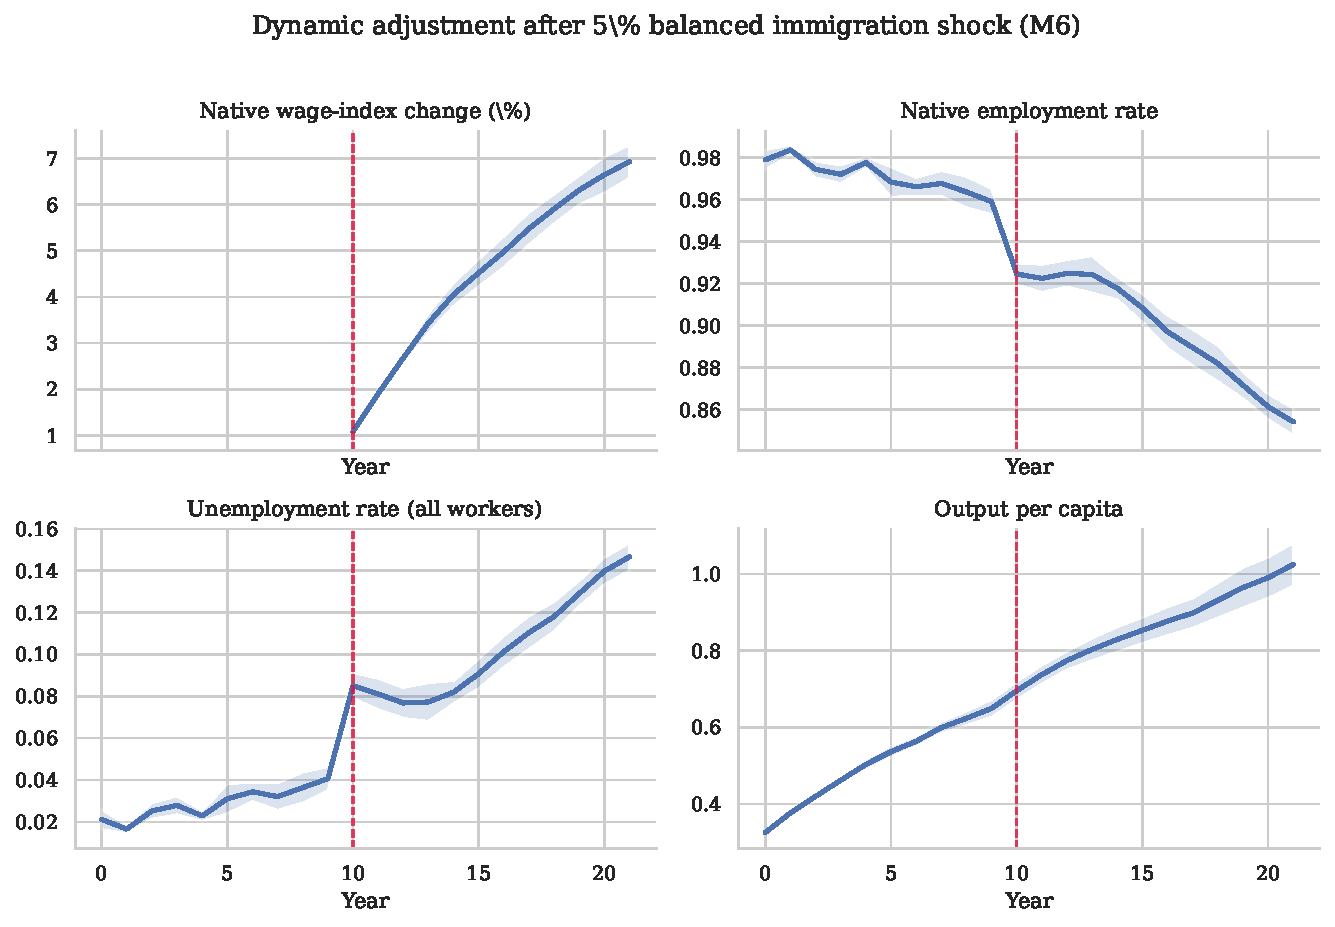
\includegraphics[width=\textwidth]{../figures/fig4_time_paths.pdf}
  \caption{Dynamic adjustment under \emph{M6} after a 5\% balanced shock (vertical line at $t=10$). Panels include unemployment; shaded bands: 95\% replicate intervals.}
  \label{fig:paths}
\end{figure}

\subsection{Heterogeneity}

Figure~\ref{fig:treatments} varies shock size, skill composition, substitutability, and macro state under \emph{M6} (eight replicates per scenario).
All scenarios yield \emph{positive} short-run wage-index changes in this parameterisation, with magnitudes between roughly 2.0 and 2.6 percentage points; unemployment rates vary only modestly across scenarios (Figure~\ref{fig:treatments}b).
Skill mix and recession timing do not generate negative average wage effects here.
The clearest heterogeneity appears in the cross-section: low-skilled natives earn lower wage-index \emph{levels} than high-skilled natives (Figure~\ref{fig:skill}), consistent with stronger substitutability at the bottom of the skill distribution \citep{dustmann2013}; the model does not report skill-specific wage \emph{changes} in the current output.

\begin{figure}[H]
  \centering
  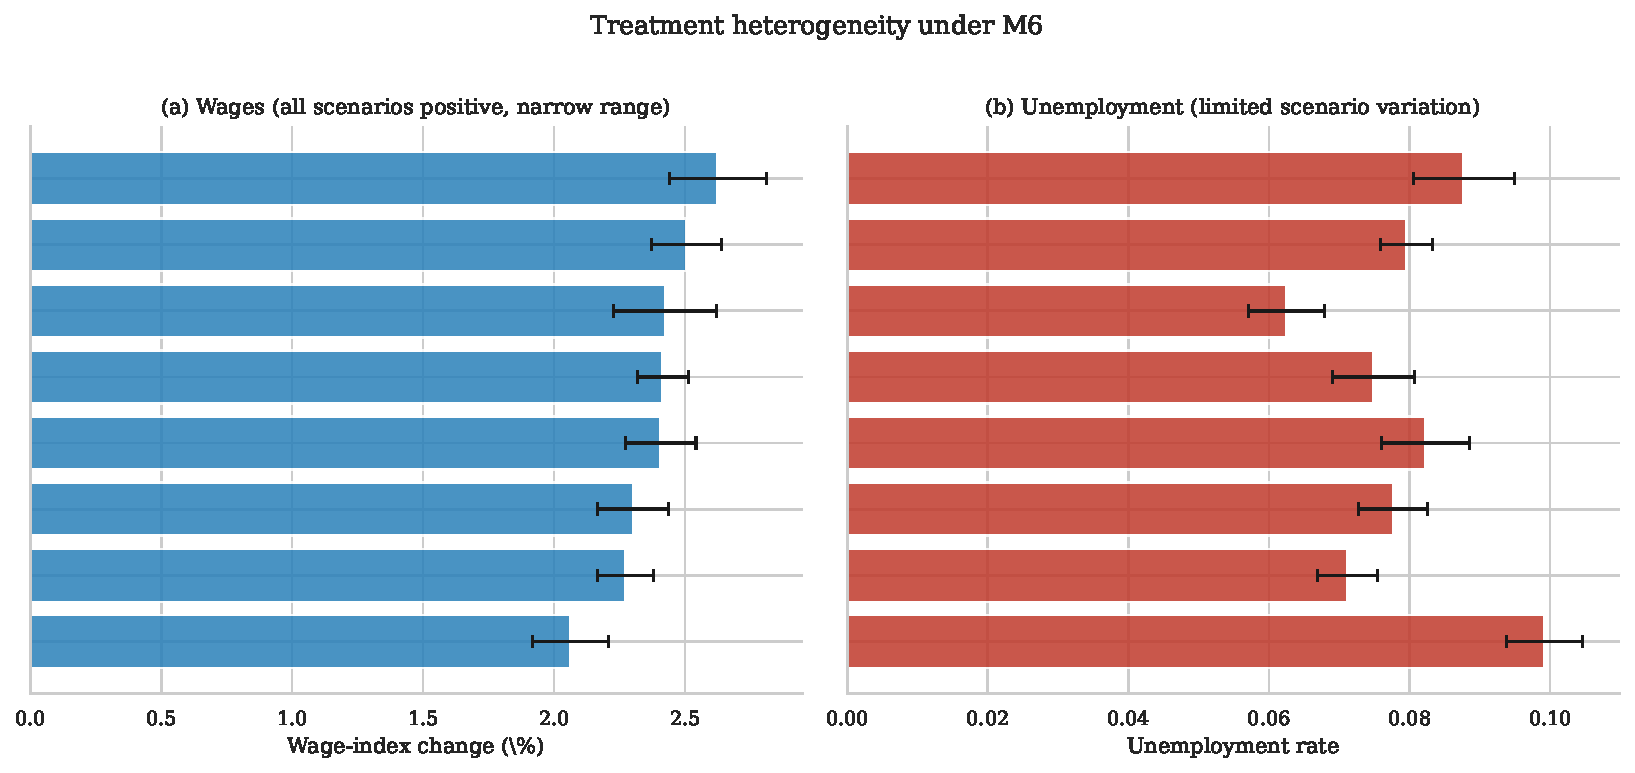
\includegraphics[width=0.92\textwidth]{../figures/fig5_treatments.pdf}
  \caption{Treatment heterogeneity under \emph{M6}: (a) short-run wage-index change; (b) short-run unemployment (8 replicates per scenario). Scenario variation is limited in this parameterisation.}
  \label{fig:treatments}
\end{figure}

Under \emph{M6}, short-run native wage-index \emph{levels} (normalised index, not percentage changes) average \LowSkillShortWage{} for low skill and \HighSkillShortWage{} for high skill---a cross-sectional gap consistent with stronger substitutability at the bottom of the skill distribution \citep{dustmann2013}.

\begin{figure}[H]
  \centering
  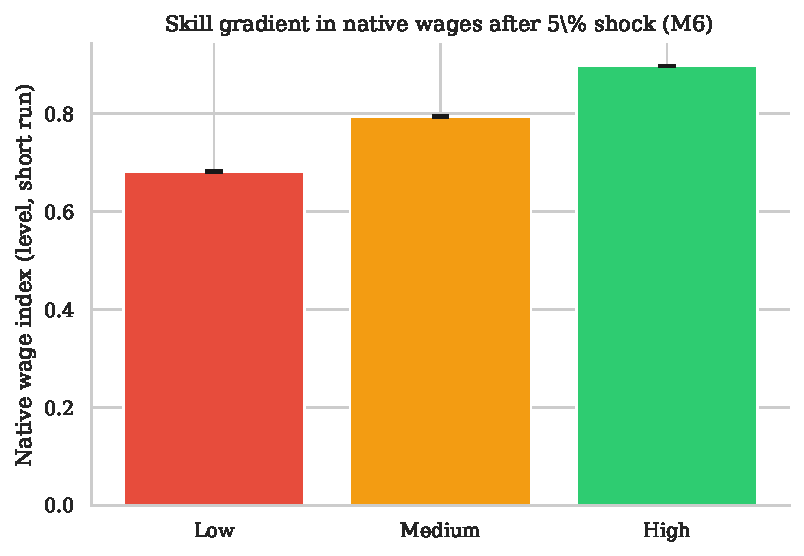
\includegraphics[width=0.72\textwidth]{../figures/fig6_skill_heterogeneity.pdf}
  \caption{Native wage-index \emph{levels} by skill tier, short run (0--2 years), \emph{M6}, 5\% shock ($N=\NReplicates{}$).}
  \label{fig:skill}
\end{figure}

\subsection{Hypothesis assessment}

\begin{table}[htbp]
  \centering
  \small
  \caption{Hypothesis assessment}
  \label{tab:hypotheses}
  \begin{tabular}{@{}clp{0.26\textwidth}@{}}
    \toprule
    & Hypothesis & Result \\
    \midrule
    H1 & Competition when margins fixed & Partial \\
    H2 & Demand attenuates/reverses wage effects & Supported \\
    H3 & Firm/capital reduces congestion & Partial \\
    H4 & Complementary natives fare better & Partial \\
    H5 & Migrant entrepreneurship & Partial \\
    H6 & Long-run wage reversal under \emph{M6} & Supported \\
    \bottomrule
  \end{tabular}
  \begin{minipage}{0.95\textwidth}
    \small\emph{Notes:} H1: \emph{M0} $\approx$ \MZeroShortWage{} pp wages, \MZeroUnempShort{}\% unemployment.
    H2: \DemandContrib{} pp at \emph{M1}.
    H3--H5: positive or negligible incremental effects; M5 $\approx 0$ pp.
    H4: skill gradient in levels (Figure~\ref{fig:skill}); weak treatment variation.
    H6: \MZeroLongWage{} $\rightarrow$ \MSixLongWage{} pp (long run).
  \end{minipage}
\end{table}

\section{Limitations and scope of inference}
\label{sec:limits}

\textbf{What this study can say.}
\begin{enumerate}[label=(\roman*), nosep]
  \item In a transparent artificial economy with stylised calibration, shutting down general-equilibrium margins yields negligible short-run wage-index changes but severe unemployment under \emph{M0}; activating demand, firm entry, and innovation can reverse the wage sign while employment dynamics remain mixed.
  \item Mechanism decomposition quantifies which margins move outcomes, helping reconcile fixed-job empirics with dynamic spatial models \citep{borjas2016,cadenakovak2016,albert2021}.
  \item Distributional predictions---a persistent skill gradient in native wage levels---are stable across replicates; differential effects by inflow skill mix are small under \emph{M6} in the current parameterisation.
\end{enumerate}

\textbf{What this study cannot say.}
\begin{enumerate}[label=(\roman*), nosep]
  \item It does \emph{not} estimate the causal effect of immigration in any real economy.
  \item Positive long-run wage effects under \emph{M6} may partly reflect stylised demand and innovation parameters rather than empirically identified magnitudes; the \emph{M0}$\rightarrow$\emph{M1} step is especially large and may be miscalibrated.
  \item Under \emph{M6}, native employment share declines over the post-shock horizon even when the wage index rises; readers should not equate higher wages with unambiguous labour-market gains for natives.
  \item Welfare institutions, collective bargaining, language policy, and housing supply are omitted.
  \item Burn-in moments need not match Table~\ref{tab:calibration} exactly; pre-shock employment under \emph{M6} is higher than the listed native-employment target.
  \item Task specialisation (\emph{M4}) and migrant entrepreneurship (\emph{M5}) contribute negligibly to the aggregate wage index in this implementation; firm entry and demand activation dominate.
  \item The model is not validated on a hold-out historical shock with pre-registered outcomes.
  \item Global sensitivity analysis and 500-replicate robustness are design targets not yet fully executed at scale.
\end{enumerate}

\textbf{Policy interpretation.}
Results caution against exporting partial-equilibrium wage estimates into long-run conclusions without stating which adjustment margins are inactive.
They do \emph{not} license a blanket claim that immigration raises wages in any specific country; they show that such a conclusion requires explicit assumptions about demand, firm creation, and productivity.

\section{Conclusion}
\label{sec:conclusion}

Immigration economics produces different answers because the underlying thought experiments differ.
This paper makes those differences explicit through a nested agent-based model in an artificial economy.
When only labour supply expands (\emph{M0}), native wage indices are essentially unchanged in the short run but unemployment rises sharply because jobs and demand are fixed.
When migrants consume locally, firms enter, capital adjusts, natives specialise, migrant entrepreneurship operates, and innovation responds (\emph{M6}), the same shock produces rising wage-index trajectories alongside a gradual decline in native employment share.

The contribution is a map from structural assumptions to signed outcomes across horizons and worker types---not a single definitive sign on ``the'' immigration effect.
Future work should embed microdata from a specific economy, validate on identified historical shocks, and conduct full sensitivity analysis at scale.

\section*{Replication and code availability}
\noindent
Source code, calibration targets, result CSVs, and figure scripts are archived at\\
\url{https://github.com/sbf-developer/migration-labour-computational-simulation}.

\smallskip\noindent
To reproduce the reported statistics and figures, run \texttt{python run\_experiment.py --replicates 50} followed by \texttt{python generate\_paper\_outputs.py}, then compile with \texttt{pdflatex} and \texttt{bibtex} in \texttt{paper/}.
All numerical values in Tables~\ref{tab:results}--\ref{tab:hypotheses} and the abstract are auto-generated from \texttt{results/mechanism\_ladder\_shock\_5pct\_balanced.csv}.

\bibliography{references}

\appendix
\section{Model schematic}
\label{app:schematic}

\begin{figure}[H]
  \centering
  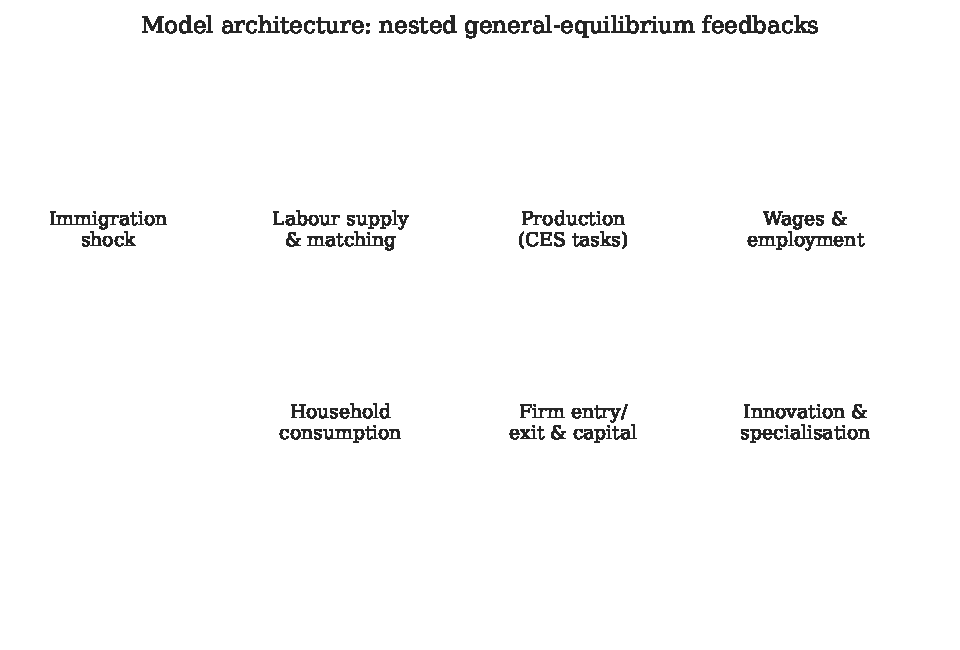
\includegraphics[width=0.88\textwidth]{../figures/fig1_schematic.pdf}
  \caption{Model architecture: nested general-equilibrium feedbacks.}
  \label{fig:schematic}
\end{figure}

\section{ODD protocol summary}
\label{app:odd}

\textbf{Purpose.} Diagnose mechanism dependence of immigration wage effects.

\textbf{Entities.} Workers, firms, implicit households.

\textbf{State variables.} Worker $(g,s,o,a,r,e,z)$; firm $(\text{sector},\text{region},A,K,\{N_{jq},M_{jq},V_{jq},w_{jq}\},p_j,\pi_j)$.

\textbf{Process overview.} Burn-in $\rightarrow$ shock at $t=10$ $\rightarrow$ adjustment with nested mechanisms.

\textbf{Design concepts.} Emergence of vacancy chains; adaptation via entry and innovation; stochastic matching.

\textbf{Initialization.} Stylised employment and wage gaps from \texttt{data/calibration\_targets.json}.

\textbf{Submodels.} Equations~\eqref{eq:production}--\eqref{eq:entry}; search protocol in Section~\ref{sec:model}.

\end{document}
